\chapter{Models on the Daily Consumption}
Now that data is cleaned and prepared, a statistical analysis consisting of data segmentation and linear regression models can be made. The purpose of the analysis is to detect which attributes affects the performance of a specific house.

\section{Linear regression}
Linear regression is a method to model the relationship between a dependent variable and one or more independent variables, where the unknown model parameters are estimated from the data. \textcolor{red}{Mangler nok lidt her.} With the dependent variable $Y$ and the independent variables $x_1, \dots, x_n$, the linear regression model is formulated as
\begin{equation}
    Y_i = \beta_0 + \beta_1 x_{i,1} + \beta_2 x_{i,2} + \cdots + \beta_p x_{i,p} + \varepsilon_i, \quad \varepsilon_i ~ \mathcal{N}(0,\sigma^2), \quad i = 1,\dots, n. \label{lm}
\end{equation}
The variables $\varepsilon_i$ are errors which are assumed to be white noise while also being i.i.d (independent and identically distributed). Equation \eqref{lm} shows a multiple linear regression model as it contains more than one explanatory variable. In this section both a simple linear model and a multiple linear model has been fitted to data given in table \ref{tab: modeldata}.

\noindent As the best linear model $Y_i$ is desired, the total deviation from the data has to be as small as possible. The least squares method given as
\begin{equation}
    \text{SSE} = \sum_{i=1}^n (Y_i - (\beta_0 + \beta_1 x_{i,1} + \beta_2 x_{i,2} + \cdots  \beta_p x_{i,p}))^2 = \sum_{i=1}^n (Y_i - \Hat{Y}_i)^2
\end{equation}
is chosen for estimating the model. The parameters $\beta_j$ are optimized to minimize the sum of squared errors of prediction (SSE).

\subsection{Model assumptions}
\noindent When SSE is minimized the model needs to be validated by checking whether the underlying model assumptions are fulfilled.
\begin{enumerate} [label=\textbf{\arabic*}]
    \item Normality of residuals
    \item Variance homogenity
    \item Variance should be independent of location
    \item Linear relationship between $x_j$ and $Y$
\end{enumerate}
Chapter 7 in \cite{Stat_bog} explains the model assupmtions listed above. To summarize, a model can be checked by looking at diagnostic plots of the residuals. The first plot considered is the Residuals vs Fitted, where the residuals are expected to be randomly scattered. To test whether the residuals are normally distributed a normal quantile–quantile plot is used. Here the residuals are expected to follow a straight line. A Scale-Location plot shows normalized and weighted residuals by sample leverage where the residuals are also expected to be randomly scattered. The last diagnostic plot shows the Residuals vs Leverage which should be a straight line and there should not be any clear patterns. If these assumptions are not met, it can influence the parameter estimates and with it the significance of the parameters. In addition, a Shapiro-Wilk test is performed to check if the residuals of the models are i.i.d with $\mathcal{N}(0,\sigma^2)$. \\

\noindent The fitting of the regression models is carried out by using the method stepwise regression which updates the model in each step. In each step it is considered whether a variable is added or subtracted from the set of explanatory variables based on specific criteria. This process is called variable selection and Chapter 7 in \cite{Stat_bog2} explains how this process can be done by using either forward or backward selection. In this project a modified version of backward selection is applied. The models are used for comparing which explanatory variables influence each house. Therefore, the models are not reduced using the \texttt{R} function \texttt{step}. Instead the signifance of the parameters are investigated and then the parameters which are significant for the majority of the houses will be used in an updated linear regression model. Thus, the variable selection is done manually which can be said to be a modified form of backward selection. The level of signifance is determined by an F-test where the variables selected have a p-value below a threshold which is chosen at 0.05. \textcolor{red}{Mangler nok en ref. til det her.}\\

\noindent Both a simple linear and a multiple linear regression model will be implemented in order to detect which attributes affect the performance of a specific house. This will be done by interpreting the estimates of the relation between the different explanatory attributes and \texttt{Consumption}. As mentioned, the p-value of the estimates of the explanatory variables will be the main focus when investigating which attributes influence the performance. Moreover, transformation of data is not considered since the purpose is to interpret the results and a transformation would \textcolor{red}{ikke gøre dette muligt eller?}

\section{Simple linear regression model}
A simple linear regression model is fitted to each house with \texttt{Consumption} as a function of \texttt{Temperature}. Since it is expected that the temperature is the physical phenomenon with the greatest influence on the heat consumption, it is chosen as the independent variable. Hence, the simple linear regression model applied to each house is
\begin{equation}
    Y_{\text{Q}} = \mu + \beta_{\text{T}} \cdot x_{\text{T}} + \varepsilon
    \label{eq: simple}
\end{equation}

\noindent The models are performed by using the \texttt{lm()} function in \texttt{R}. The models will then be validated by examining whether the model assumptions in Chapter 4.1.1 are met and different tests on normality of residuals are perfomed. The simple model only includes one explanatory variable, thus a variable selection is not performed. \textcolor{red}{Synes der mangler et eller andet her}

\subsection{Validation}
To validate the model, different methods are used. The abovementioned model assumptions are checked and futhermore tests of normally distributed residuals is performed. If the model assumptions are fulfilled and the residuals are i.i.d with $\mathcal{N}(0,\sigma^2)$, the model is said to be valid. \\

\noindent \cref{fig: simple_lm_18} and \cref{fig: simple_lm_55} shows examples of the model applied on two of the houses, where one does not fulfill the assumptions and another model that overall can be said to fulfill the assumptions. The Residuals vs. Fitted plot in \cref{fig: simple_lm_18} clearly shows that the residuals are not randomly scattered around mean 0 indicating that the variance are not constant and an odd behaviour appears in the bottom left corner. The QQ-plot shows tails and the residuals do not follow a straight line. The Scale-Location and Residuals vs. Leverage plots also show that the residuals can not be said to be i.i.d. In contrast to the model of house 18, the behavior of the residuals in \cref{fig: simple_lm_55} seems more normally distributed. Overall, they are randomly scattered around mean 0 and the QQ-plot shows that the majority  of the residuals lie on a straight line. However, the majority of the models do not fulfill the assumptions.
\begin{figure}
    \centering
    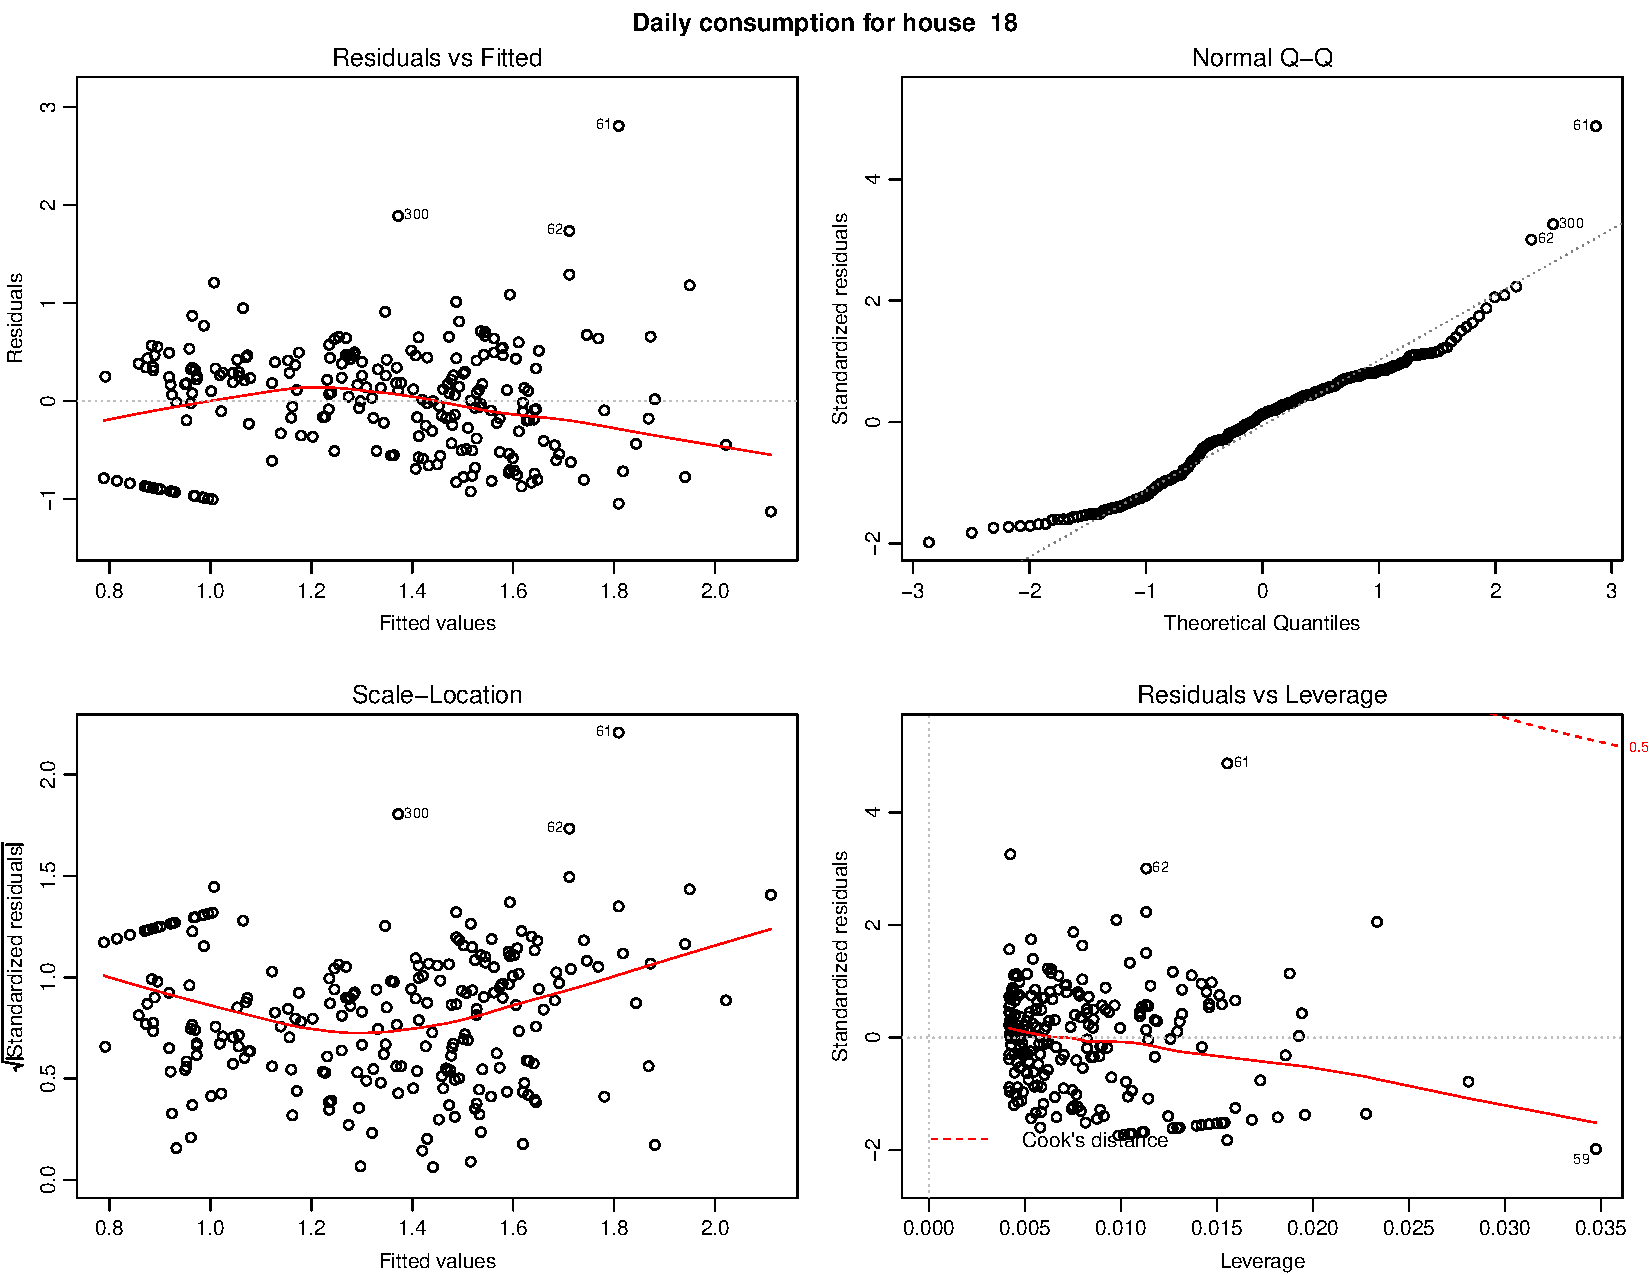
\includegraphics[width=1.\textwidth]{../../../figures/simple_lm18.pdf}
    \caption{Residual plots of house 18 based on the simple linear regression model given in \cref{eq: simple}. The model assumptions of a linear regression model are not fulfilled for this specific house}
    \label{fig: simple_lm_18}
\end{figure}
\begin{figure}
    \centering
    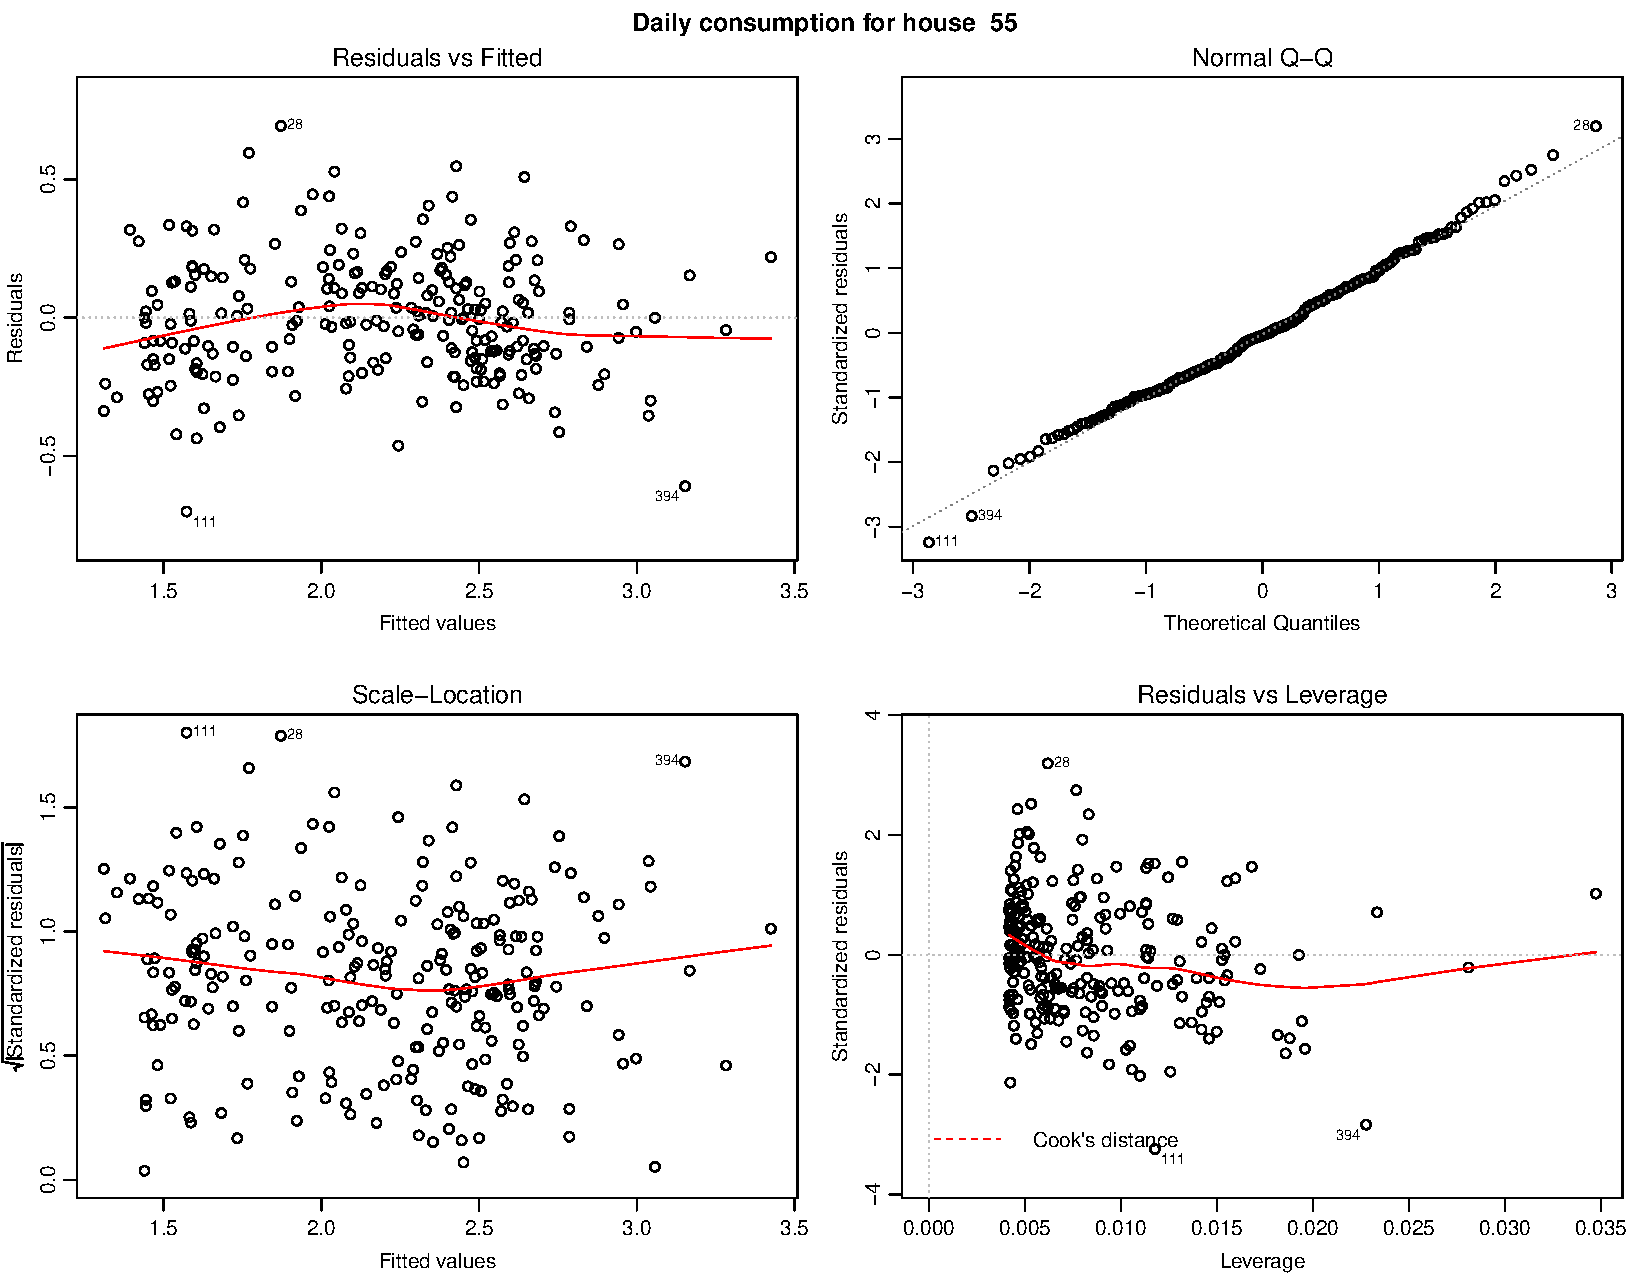
\includegraphics[width=1.\textwidth]{../../../figures/simple_lm55.pdf}
    \caption{Residual plots of house 55 based on the simple linear regression model given in \cref{eq: simple}. The model assumptions of a linear regression model are overall fulfilled}
    \label{fig: simple_lm_55}
\end{figure}
In addition, a Shapiro-Wilk test and a sign test is perfomed. The hypothesis tested in the Shapiro-Wilk test is that the residuals are i.i.d and if the p-value $> 0.05$ the hypothesis can not be rejected i.e. the residuals are normally distributed. In the sign test the hypothesis is that the number of positive signs are equal to the number of negative signs, which is one of the requirements when checking for normality. If the model assumptions are also fulfilled, then the model is concluded to be valid. The p-values from both of the tests are found in \cref{tab: shapiro_simple_lm} and it is clearly seen that the majority of the simple linear regression models have residuals with p-value above the significance level at 0.05. Thus, the hypothesis is rejected and it can be concluded that the residuals are not i.i.d.
% \textcolor{blue}{Det interessante at kigge efter er de huse, hvis residuals har en mærkværdig opførsel eller den simple modellering. Som eksempel ses hus 18 i figur \ref{fig: simple_lm_18}. Det ses tydeligt, at residualerne for modellen for dette specifikke hus er gakket. Q-Q plottet ligger ikke fint langs en ret linje. Residuals vs. fitted viser en underlig opførsel, som ikke er randomly scattered.}

\subsection{Results}
\cref{tab: est_simple_lm} shows the estimates from all the simple linear regression models and they are also visualized in \cref{fig: } including a 95\% confidence interval.

\noindent \textcolor{blue}{Overordnet kan den simple lineære regressionsmodel ikke beskrive trenden. Den antager, at temperaturen er den eneste faktor der påvirker husenes varmeforbrug. Men ved at undersøge hvorvidt model assumptions er opfyldt, så 'failer' modellen i de fleste tilfælde. Dette tyder på, at der findes flere faktorer, der påvirker varmeforbruget, hvilket selvfølgelig er forventet. Der vendes tilbage til dette i sammenligningen af de to regressionsmodeller. Når vi fitter en lineær model med en attribute, så vil man lægge linjen så summen af alle residualerne er lig 0, derfor består sign testen, men shapiro og model assumptions er ikke opfyldt, så det er ikke nok.}

The conclusion that the temperature is highly significant implies that this attribute will be included in the multiple linear regression model.

\section{Multiple linear regression model}
The linear regression model is extended to a multiple linear regression model as the inclusion of several independent variables is expected to improve the model. The simple model clearly showed that the heat consumption is affected by other physical factors than temperature. Hence, a full multiple linear regression model containing the attributes given in Table \ref{tab: modeldata} is performed on the model data. The backward selection of the variables are perfomed such that the highly significant parameters from the full multiple regression model are chosen and used to develop an updated model. Since \texttt{Condition} and \texttt{PrecipitationProbability} are not normalised, they are excluded from the model. In addition, it is mentioned in Chapter 2 that the house data consists of house with observations for approximately a year and house with observations for approximately six months. Thus, the two distinct lengths of observations are modeled slighty different. There do not exist observations for winter break and spring break in the data containing the short houses. The parameters will be denoted as follows: Intercept (I), Temperature (T), North (N), East (E), South (S), West (W), Mean Sea Level (MSL), Solar Radiation (SR), Winter Break (WB), Spring Break (SB), Autumn Break (AB), Christmas Break (CB), Weekend (WKND), the interaction between the temperature and the different wind directions (T:N, T:E, T:S, T:W). This lead to the following two multiple linear regression models:
\begin{align}
    Y_{Q,L} = \mu & + \beta_{\text{T}}\cdot x_{\text{T}} + \beta_{\text{N}}\cdot x_{\text{N}} + \beta_{\text{E}}\cdot x_{\text{E}}+ \beta_{\text{S}}\cdot x_{\text{S}} + \beta_{\text{W}}\cdot x_{\text{W}} + \beta_{\text{MSL}}\cdot x_{\text{MSL}} \nonumber \\ & + \beta_{\text{SR}}\cdot x_{\text{SR}} + \beta_{\text{WB}}\cdot x_{\text{WB}} + \beta_{\text{SB}}\cdot x_{\text{SB}}  + \beta_{\text{AB}}\cdot x_{\text{AB}} + \beta_{\text{CB}}\cdot x_{\text{CB}} \label{eq: multi_L}  \\ & + \beta_{\text{WKND}}\cdot x_{\text{WKND}} + (\beta_{\text{T:N}} + \beta_{\text{T:E}} + \beta_{\text{T:S}} + \beta_{\text{T:W}}) \cdot x_{\text{T}} + \varepsilon \nonumber \\ \nonumber \\
    Y_{Q,S} = \mu & + \beta_{\text{T}}\cdot x_{\text{T}} + \beta_{\text{N}}\cdot x_{\text{N}} + \beta_{\text{E}}\cdot x_{\text{E}}+ \beta_{\text{S}}\cdot x_{\text{S}} + \beta_{\text{W}}\cdot x_{\text{W}} + \beta_{\text{MSL}}\cdot x_{\text{MSL}} \nonumber \\ & + \beta_{\text{SR}}\cdot x_{\text{SR}} + \beta_{\text{AB}}\cdot x_{\text{AB}} + \beta_{\text{CB}}\cdot x_{\text{CB}} + \beta_{\text{WKND}}\cdot x_{\text{WKND}} \label{eq: multi_S} \\ & + (\beta_{\text{T:N}} + \beta_{\text{T:E}} + \beta_{\text{T:S}} + \beta_{\text{T:W}}) \cdot x_{\text{T}} + \varepsilon  \nonumber
\end{align}
The models include the interaction between the temperature and the wind since it is expected that this interaction has an influence on the heat consumption. That is, it is expected that the influence of the wind is greater when the temperature is lower. In linear regression, it is desired to have as simple a model as possible, and since the models would be too complex when including all the interactions, only the interaction between the temperature and the wind is included.\\

\noindent The models show that the interactions between the attribute \texttt{Holiday} and the other attributes are chosen to be excluded. The reason is that \texttt{Holiday} is used to investigate how the consumption changes during holiday periods. The parameters will be denoted as follows: Intercept (I), Temperature (T), North (N), East (E), South (S), West (W), Mean Sea Level (MSL), Solar Radiation (SR), Winter Break (WB), Spring Break (SB), Autumn Break (AB), Christmas Break (CB), Weekend (WKND) and the interaction between the temperature and the different wind directions (T:N, T:E, T:S, T:W). The wind directions are not inserted directly into the model. As mentioned in \cref{tab: weatherdata}, the wind directions are given as degrees from $0$ to $360$. Instead of just classifying degree intervals as north, south, east or west, splines are used to model the directions. How this is done is described below.
\noindent As for the simple model, the multiple models must also be validated by investigating diagnostic plots and testing for normally distributed residuals. Before performing the models, the wind will be modified which the following section explains.

\noindent The models show that the interactions between the attribute \texttt{Holiday} and the other attributes are chosen to be excluded. The reason is that \texttt{Holiday} is used to investigate how the consumption changes during holiday periods. The parameters will be denoted as follows: Intercept (I), Temperature (T), North (N), East (E), South (S), West (W), Mean Sea Level (MSL), Solar Radiation (SR), Winter Break (WB), Spring Break (SB), Autumn Break (AB), Christmas Break (CB), Weekend (WKND) and the interaction between the temperature and the different wind directions (T:N, T:E, T:S, T:W). The wind directions are not inserted directly into the model. As mentioned in \cref{tab: weatherdata}, the wind directions are given as degrees from $0$ to $360$. But in the model the wind direction is not quantified in this way, rather it should be an effect on each of the four major directions: north, south, east and west. These will in the following be called wind direction categories. One way to classify the wind direction could be to use indicator variables, and assign each possible wind direction to a category. In this project spline functions will be used to determine the effect a certain wind direction has on the categories. As a consequence, a wind direction can have different effects on different categories. For example wind coming directly from north might have a large effect on the north category, but also a lesser effect on east and west. In real life the wind direction is often distorted close to the ground because of turbulence. Also wind directions on the border between two categories should have an effect on both. For these reasons, splines seem like a good choise for modelling the wind.

\subsection{Splines}
Each major direction is described by a basis spline. Together they form a spline basis, that spans the space of the wind direction. The theory on splines introduced here is based on \cite{Splines}. A spline basis is defined by a knot vector $\Xi$ and a polynomial degree $q\in \mathbb{N}$. The i'th basis spline is a function $\mathcal{N}^q_{\Xi,i}: \mathbb{R} \rightarrow \mathbb{R}$. If the spline basis should contain $n$ basic splines, then $\Xi=\{\xi_1, \xi_2,...,\xi_{n+q+1}\}$. When the knots are equidistant, the spline is uniform. Then the spline is defined by the Cox-de Boor recursion formula:

\begin{equation}
    \mathcal{N}_{\Xi,i}^0 (\xi) =
    \begin{cases}
    1 \quad \text{if} \ \ \xi_i \leq \xi \leq \xi_{i+1}\\
    0 \quad \text{otherwise}\,,
    \end{cases}
\end{equation}
for the splines of degree $0$, and for higher degrees
    \begin{equation}
        \mathcal{N}_{\Xi,i}^j(\xi) = \frac{\xi-\xi_i}{\xi_{i+j}-\xi_i}\mathcal{N}_{\Xi,i}^{j-1}(\xi) + \frac{\xi_{i+j+1}-\xi}{\xi_{i+j+1}-\xi_{i+1}} \mathcal{N}_{\Xi, i + 1}^{j-1}(\xi),
    \end{equation}
for $j=1,2,..,q$ and $i=1,2,...,n+q-j$. When the splines are uniform, the continuity of the basis splines across a knot is $q-1$. This means that the $q-1$'th derivative exists and is continuous. In this project splines of degree $2$ is used, meaning that the first derivative is continuous at every point on the spline. The splines used here are periodic. that means that after the first $n$ knots, the knot sequence starts over. For modelling the wind direction, four knots are used for the knot vector, each associated with a wind direction category.  Here they are defined as $northeast$, $southeats$, $southwest$ and $northwest$. The reason for this will be explained later in this section. For each of these knots there is a basis spline. When the degree of the splines is $2$, it means that the spline for a given knot is zero at the opposite knot. For example, when using four knots the spline peaking in the north would always be zero in the south. Higher degrees would not maintain this property. The spline basis can be seen on \cref{fig:spline_basis}. Notice that the sum of the entire spline basis at a given point always adds up to one. The figure shows how the $i$'th spline, associated with the $i$'th knot does not peak at that knot, but in the following interval. This is the reason why the knots are chosen in this way. By choosing the knots to be between the main directions north, east, south and west, this is where the basic splines peek.



\begin{figure}
    \centering
    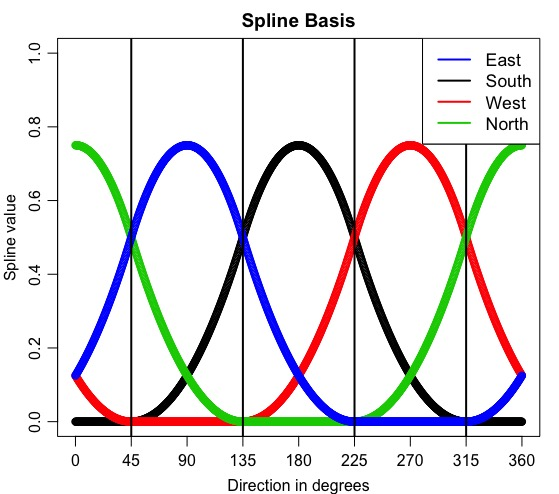
\includegraphics[width=0.8\textwidth]{../../../figures/SplineBasis.jpeg}
    \caption{The spline basis used to model the wind direction. Each color is a different basis spline, and the vertical lines mark the knots}
    \label{fig:spline_basis}
\end{figure}

Now the splines can be used to represent their category in the linear regression model. At a given data point, the wind direction is given as input to each basic spline. The result is then weighted by the windspeed. The result is used as the effect of the effect of the category that spline represents. As an example, a windspeed of $2$ from the angle $135$ degrees would give the following result for the variables in the regression model: $x_N=0$, $x_E=0.5$, $x_S=0.5$ and $x_W=0$. These results can be derived from \cref{fig:spline_basis}.



%\subsection{Validation}
%The multiple models has to fulfill several assumptions.


%\begin{figure}
%    \centering
%    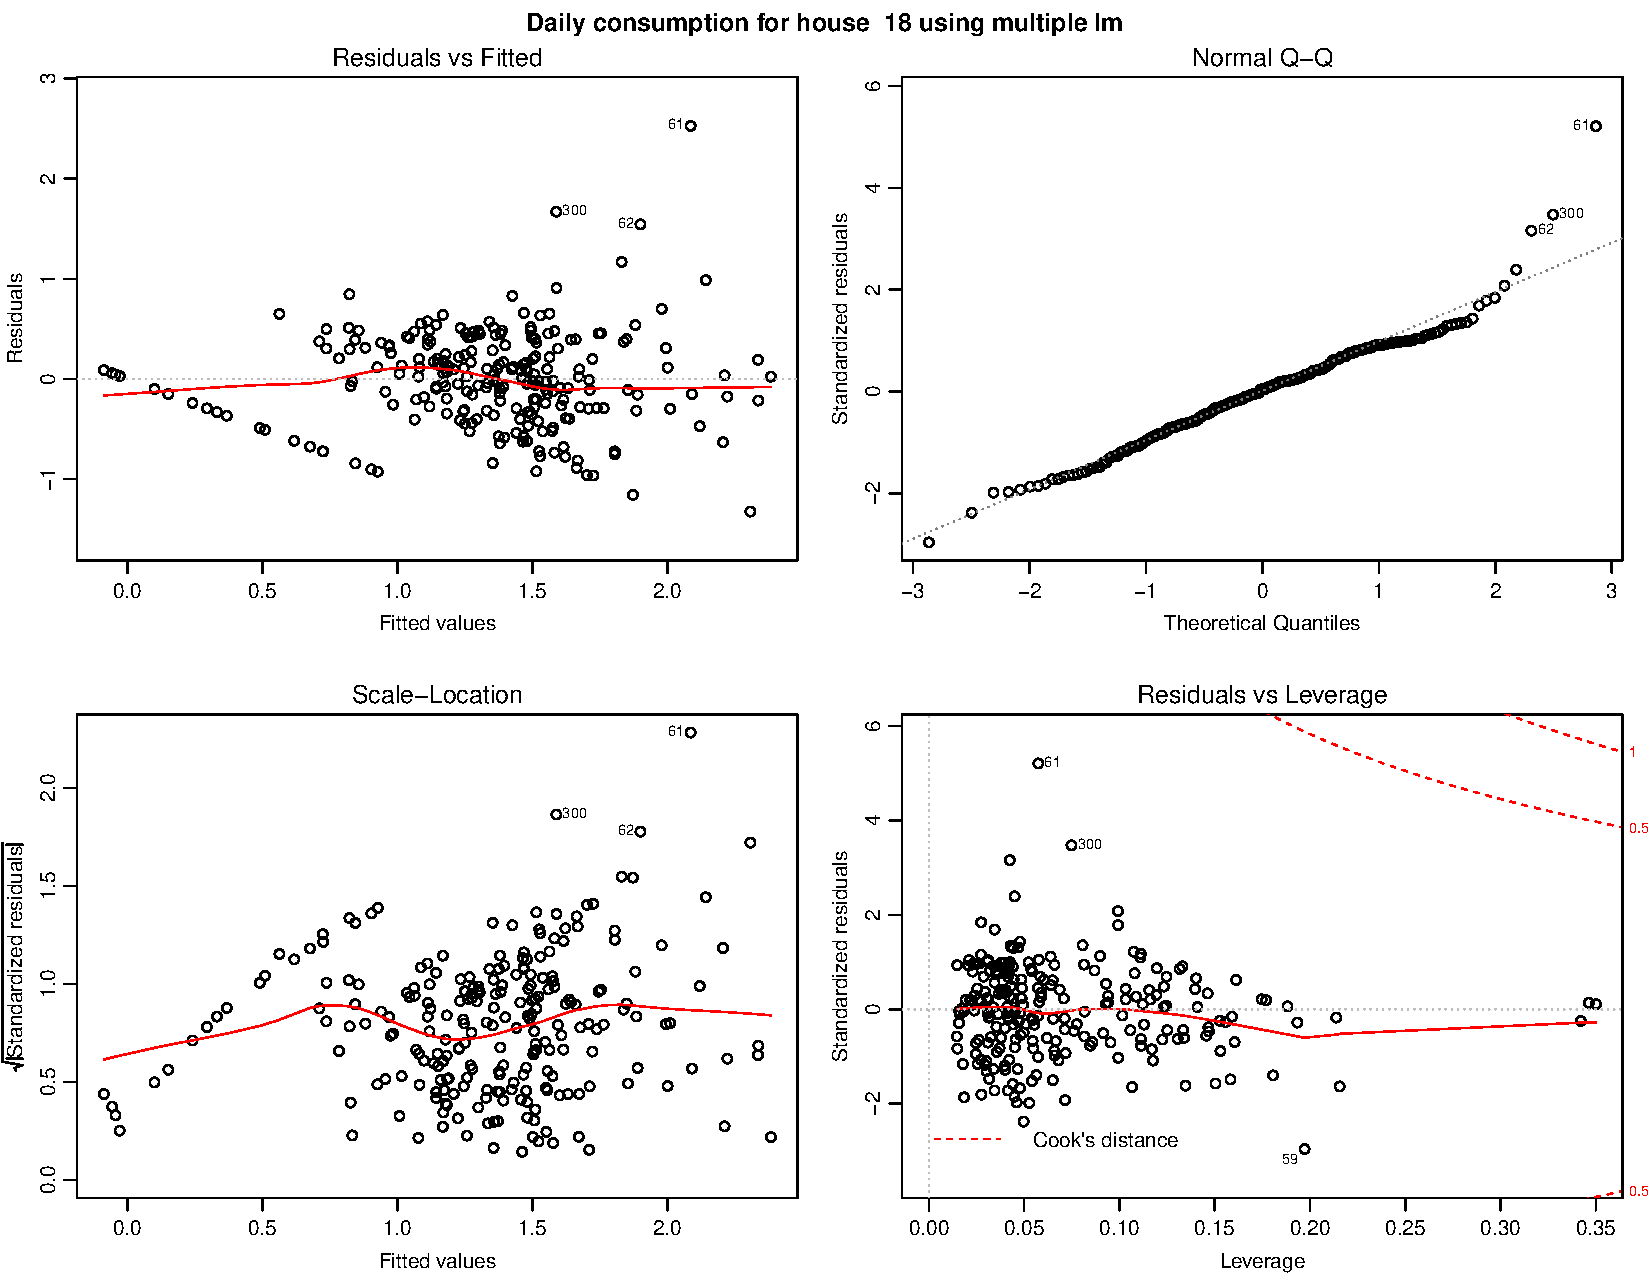
\includegraphics[width=1.\textwidth]{../../../figures/multiple_lm18L.pdf}
%    \caption{Diagnostic plot of the multiple linear regression model for long house 18}
%    \label{fig: multiple_lm18L}
%\end{figure}
%\begin{figure}
%    \centering
%    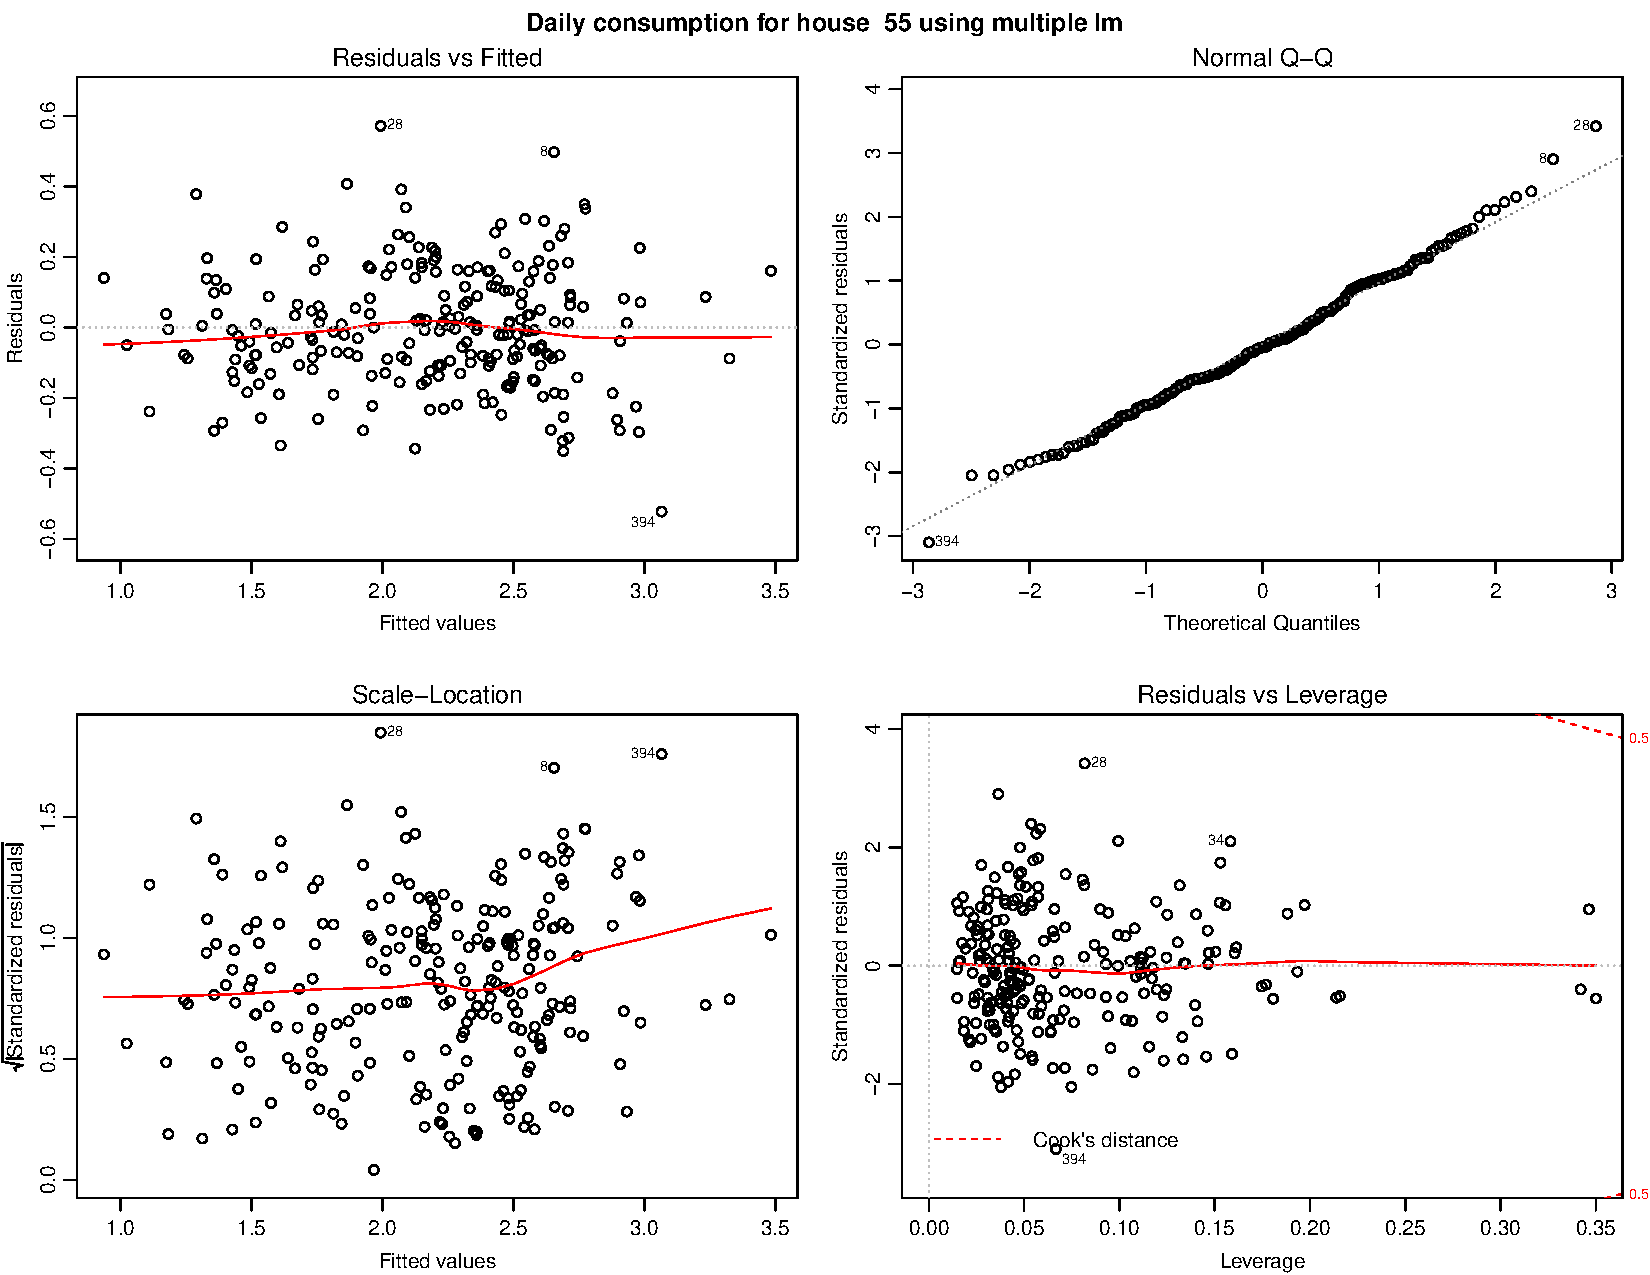
\includegraphics[width=1.\textwidth]{../../../figures/multiple_lm55L.pdf}
%    \caption{}
%    \label{fig: multiple_lm55L}
%\end{figure}


%\begin{figure}
%    \centering
%    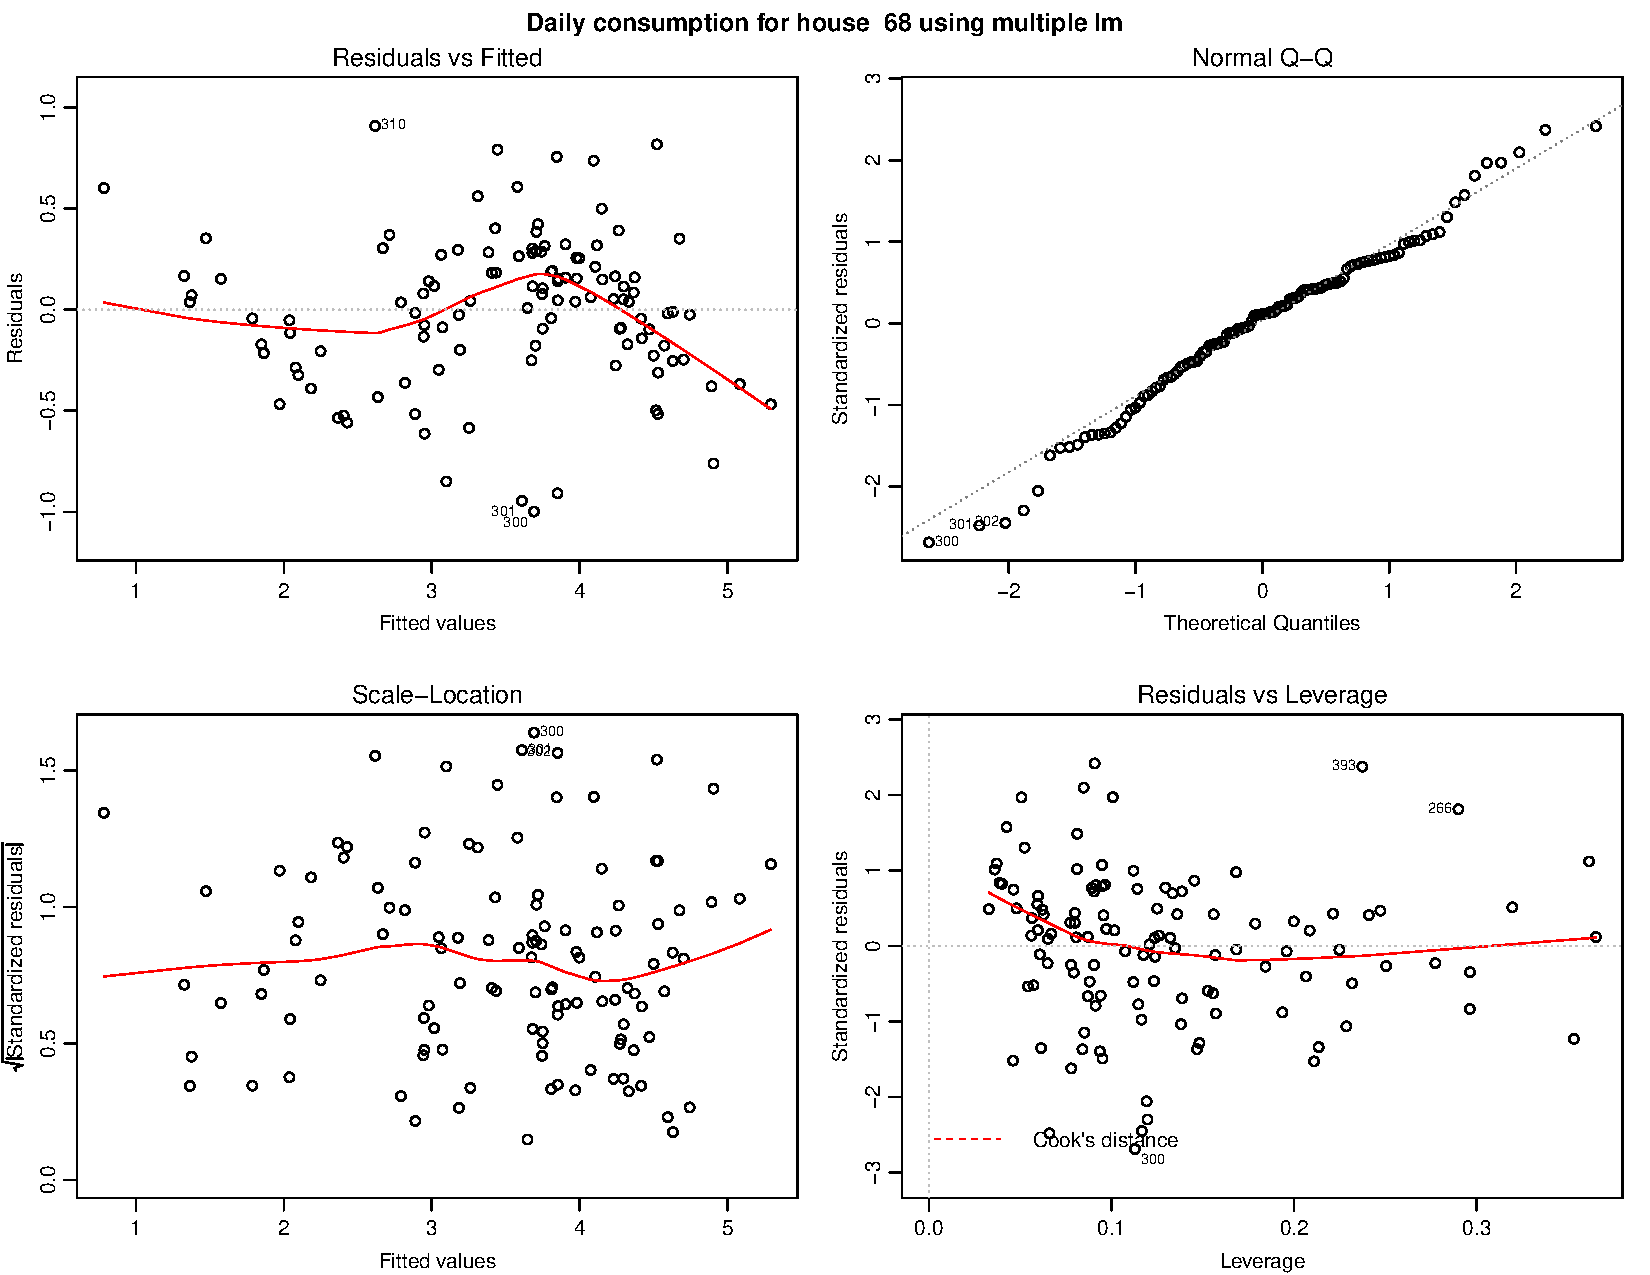
\includegraphics[width=1.\textwidth]{../../../figures/multiple_lm68S.pdf}
%    \caption{}
%    \label{fig: multiple_lm68S}
%\end{figure}


\subsection{Results}
The full multiple regression models are steps of the backward selection which is why they are not validated. The purpose of this step is, as mentioned, to determine which parameters are found to be significant in the majority of the models. Hereafter, these parameters are included in a general regression model that can be used for comparing the houses performance.

\noindent When performing the two models given in \cref{eq: multi_L} and \cref{eq: multi_S}, without reduction, the significance of the parameters are determined and can be found in \cref{tab: lmMult_full_L}-\ref{tab: lmMult_full_S}. In addition, \cref{tab: lmMult_full_L_sum} and \cref{tab: lmMult_full_S_sum} are generated in order to determine which parameters are significant for the majority of the houses. The tables clearly show that the total of significance of each parameter for the different holidays occurs in less than half of the cases.

\textcolor{red}{Hvis bare én af retningerne har over halvdelen signifikant skal alle retningerne med.}

\begin{table}
    \centering
    \resizebox{0.70\textheight}{!}{\begin{tabular}{l|cccccccccccccccccccc}
     \hline
    & I & T & N & E & S & W & MSL & SR & WB & SB & AB & CB & WKND & T:N & T:E & T:S & T:W \\
    \hline
    Sum of *** & 5 & 41 & 0 & 18 & 2 & 24 & 6 & 22 & 3 & 3 & 1 & 5 & 4 & 0 & 1 & 7 &9 \\
    Sum of ** & 6 & 1 & 1 & 9 & 5 & 12 & 4 & 10 & 6 & 2 & 0 & 2 & 0 & 1 & 1 & 9 & 9 \\
    Sum of * & 6 & 1 & 5 & 7 & 7 & 2 & 2 & 2 & 3 & 6 & 5 & 3 & 8 & 2 & 3 & 5 & 11 \\
    \hdashline
    Total of 43 & 17 & 43 & 6 & 34 & 14 & 38 & 12 & 34 & 12 & 11 & 6 & 10 & 12 & 3 & 5 & 21 & 29 \\
    \hline
\end{tabular}}
\caption{The distribution of significant parameters from the multiple linear regression model for long houses. There are 43 long houses, thus the total of the signifance of each parameter for each house is in relation to the number of long houses}
\label{tab: lmMult_full_L_sum}
\end{table}
\begin{table}
    \centering
    \resizebox{0.7\textheight}{!}{\begin{tabular}{l|cccccccccccccccccc}
     \hline
    & I & T & N & E & S & W & MSL & SR & AB & CB & WKND & T:N & T:E & T:S & T:W \\
    \hline
    Sum of *** & 0 & 27 & 0 & 4 & 0 & 15 & 0 & 5 & 2 & 0 & 0 & 0 & 0 & 0 & 3\\
    Sum of ** & 2 & 0 & 0 & 6 & 2 & 5 & 2 & 6 & 0 & 0 & 3 & 0 & 0 & 2 & 5 \\
    Sum of * & 2 & 0 & 1 & 8 & 4 & 4 & 4 & 4 & 2 & 5 & 2 & 1 & 1 & 3 & 9 \\
    \hdashline
    Total of 27 & 4 & 27 & 1 & 18 & 6 & 24 & 6 & 15 & 4 & 5 & 5 & 1 & 1 & 6 & 17\\
    \hline
\end{tabular}}
\caption{The distribution of significant parameters from the multiple linear regression model for short houses. As for the long houses, the total of the signifance is in relation to the number of long houses}
\label{tab: lmMult_full_S_sum}
\end{table}




\section{Regression model for comparing houses}
Based on the tables illustrating the significant parameters for the long and short houses, an updated multiple linear regression model is made. The purpose of this more general model is to compare which parameters influence each house. Furthermore, houses with e.g. same area, construction year etc. can be compared. The comparison model derived from \cref{tab: lmMult_full_L_sum} and \cref{tab: lmMult_full_S_sum}, becomes
\begin{align}
        Y_{Q} = \mu & + \beta_{\text{T}}\cdot x_{\text{T}} + \beta_{\text{N}}\cdot x_{\text{N}} + \beta_{\text{E}}\cdot x_{\text{E}}+ \beta_{\text{S}}\cdot x_{\text{S}} + \beta_{\text{W}}\cdot x_{\text{W}} \nonumber \\ & + \beta_{\text{SR}}\cdot x_{\text{SR}} + (\beta_{\text{T:N}} + \beta_{\text{T:E}} + \beta_{\text{T:S}} + \beta_{\text{T:W}}) \cdot x_{\text{T}} + \varepsilon. \label{eq: general_lm}
\end{align}
Likewise, the models are validated and if the assumptions are fulfilled \textcolor{red}{Et eller andet her.}

\subsection{Validation}
In order to determine whether the general model is valid, the diagnostic plots in \cref{fig: general_lm18L} and \cref{fig: general_lm55L} are investigated. The residuals from the model for house 18 behave quite odd and are not randomly scattered. It seems like this specific house can not be described by a linear regression model, which will be discussed further in Chapter \textcolor{red}{diskussionen}. On the other hand, the diagnostic plots of the residuals from house 18 are definitely improved and the residuals show a randomly behavior. Furthermore, the Shapiro-Wilk tests and the sign tests in \cref{tab: shapiro_multiple_lm} is used to determine if the general model is valid.
\begin{figure}
    \centering
    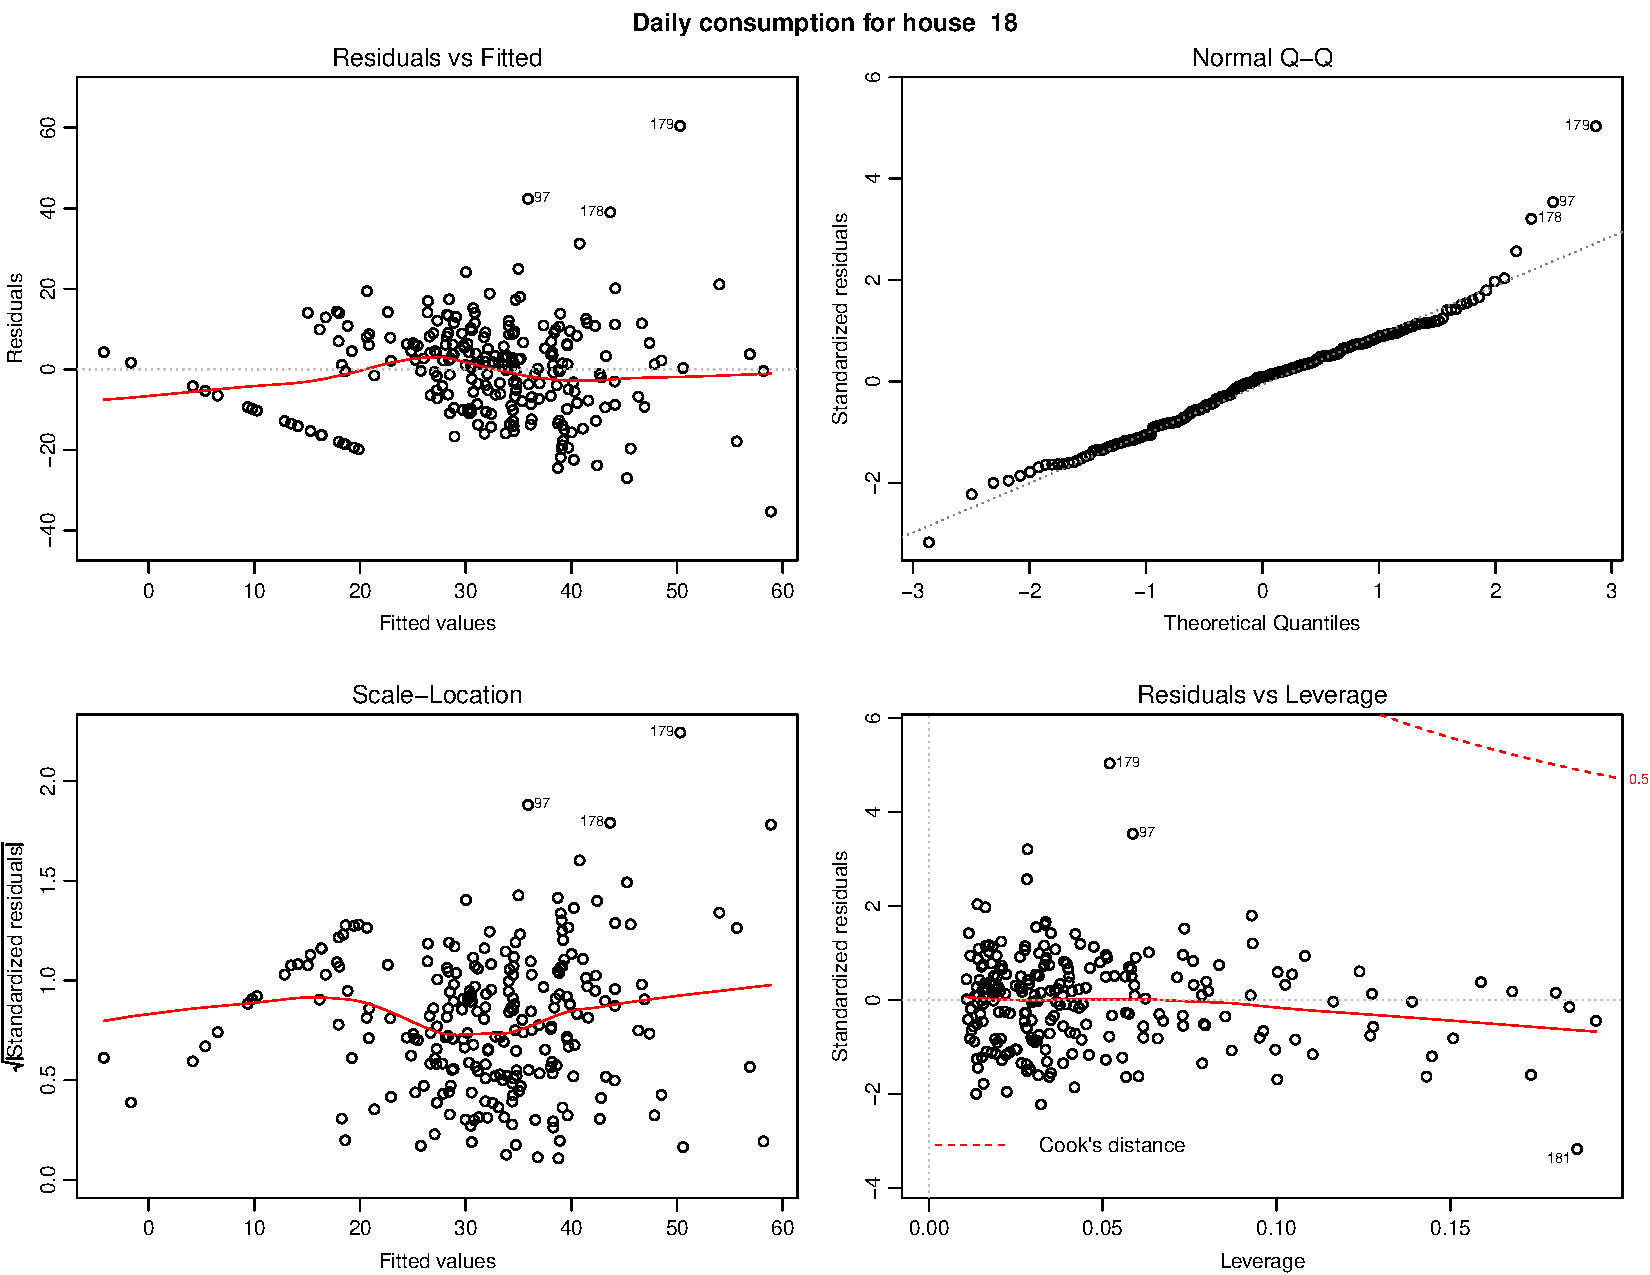
\includegraphics[width=1.\textwidth]{../../../figures/general_lm18L.pdf}
    \caption{Diagnostic plot of the general multiple linear regression model for long house 18}
    \label{fig: general_lm18L}
\end{figure}
\begin{figure}
    \centering
    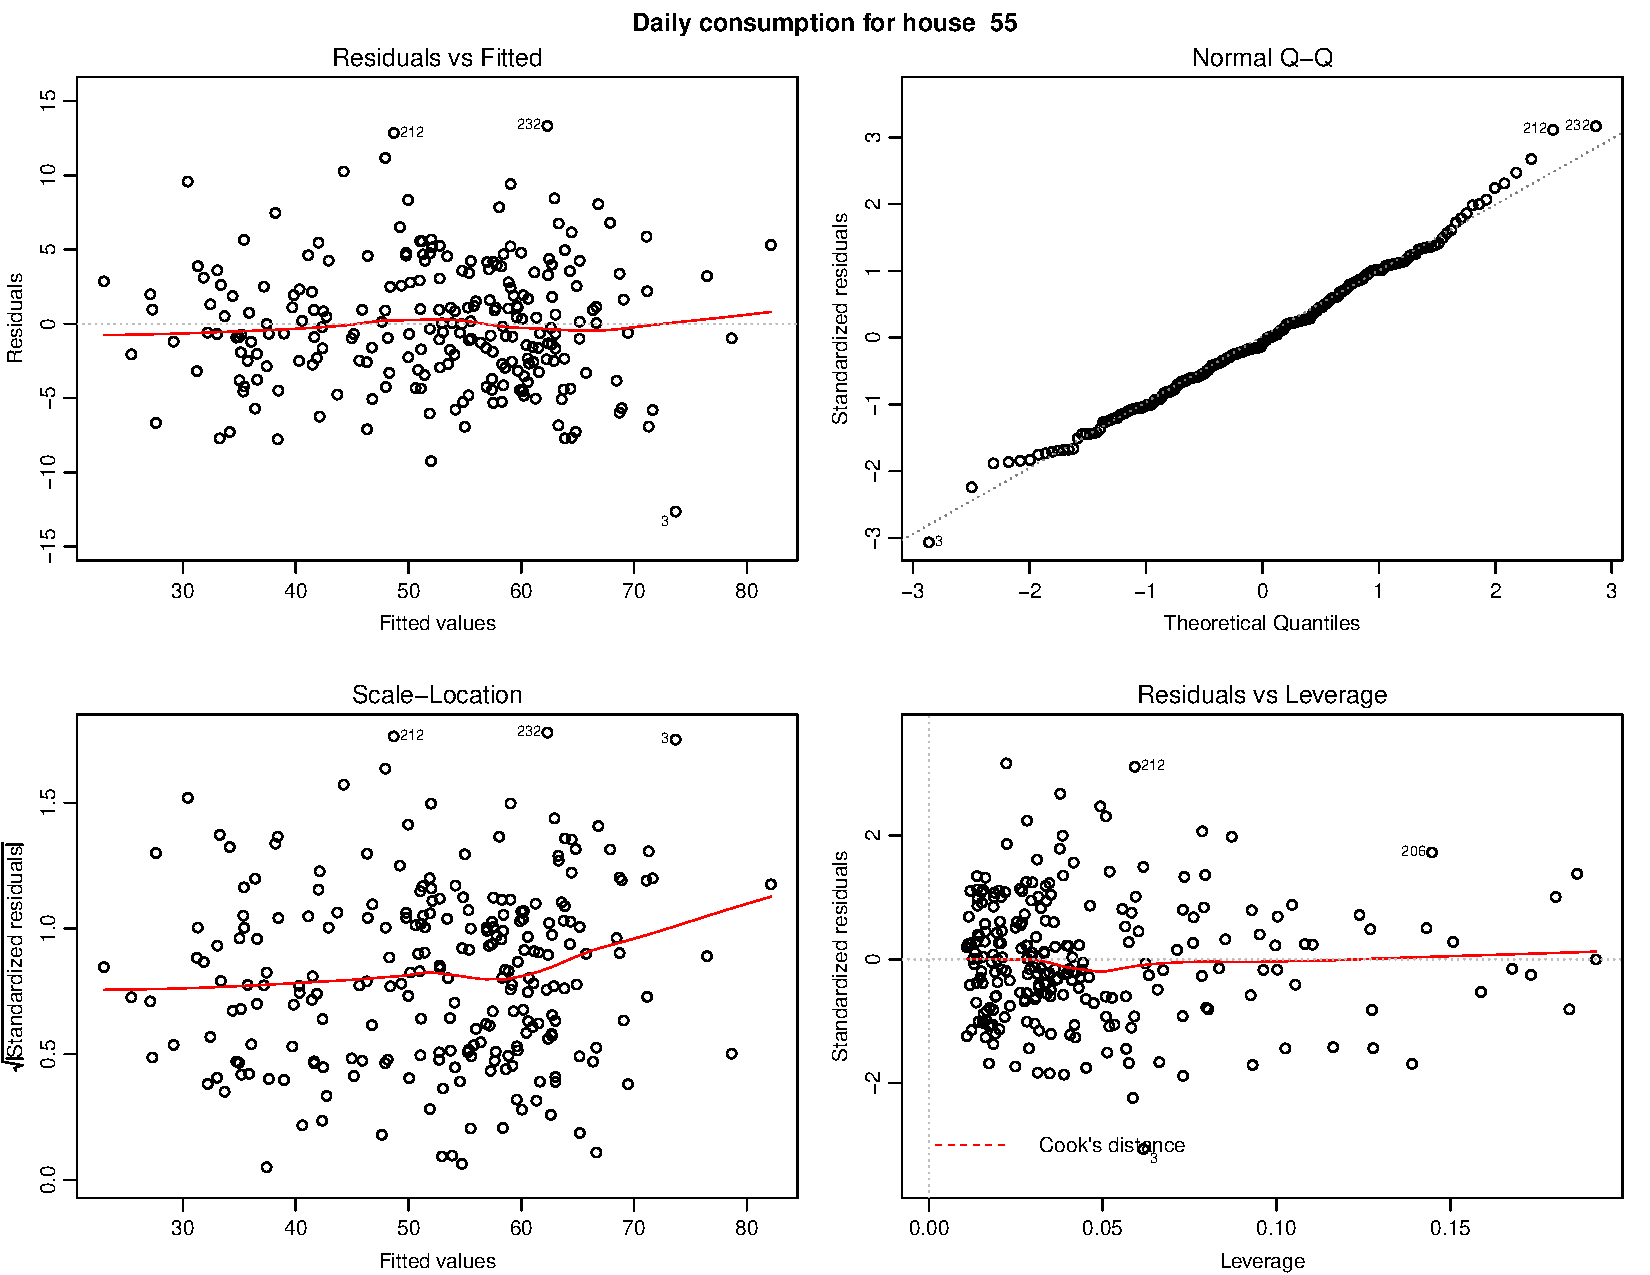
\includegraphics[width=1.\textwidth]{../../../figures/general_lm55L.pdf}
    \caption{Diagnostic plot of the general multiple linear regression model for long house 55}
    \label{fig: general_lm55L}
\end{figure}


\subsection{Results}
\begin{table}
    \centering
    \begin{tabular}{cccccccccccc}
     \hline
     Index & I & T & N & E & S & W & SR & T:N & T:E & T:S & T:W \\
    \hline
    1& \Plus *** & \Minus *** &  &  &  & \Plus ** &  &  &  & \Plus . & \Minus ** \\
2& \Plus *** & \Minus *** &  & \Plus ** &  & \Plus *** & \Minus *** &  &  &  & \Minus *** \\
3& \Plus *** & \Minus *** &  & \Plus *** &  & \Plus *** & \Minus *** &  &  & \Plus * & \Minus * \\
4& \Plus *** & \Minus *** & \Plus * &  & \Plus *** &  & \Minus *** &  &  &  &  \\
5& \Plus *** & \Minus *** &  & \Plus *** &  & \Plus *** & \Minus *** & \Plus * &  & \Plus *** & \Minus ** \\
7& \Plus *** & \Minus *** & \Minus ** & \Plus *** & \Minus . & \Plus ** & \Plus *** &  & \Minus ** & \Plus * & \Minus ** \\
11& \Plus *** & \Minus *** &  & \Plus *** &  & \Plus *** & \Minus *** &  &  & \Plus * &  \\
12& \Plus *** & \Minus *** &  & \Plus . &  & \Plus * &  &  &  &  &  \\
14& \Plus *** & \Minus *** &  & \Plus *** &  & \Plus *** & \Minus ** &  &  & \Plus ** &  \\
18& \Plus *** & \Minus ** &  & \Plus *** & \Minus ** & \Plus ** & \Plus . &  &  & \Plus *** & \Minus *** \\
21& \Plus *** & \Minus *** &  & \Plus * &  & \Plus *** &  &  &  &  & \Minus *** \\
22& \Plus *** & \Minus *** &  &  & \Plus *** & \Plus ** & \Minus *** &  &  &  & \Minus * \\
23& \Plus *** & \Minus *** & \Minus . & \Plus * &  & \Plus *** & \Minus *** &  &  & \Plus *** & \Minus *** \\
28& \Plus *** & \Minus *** &  & \Plus * & \Plus . &  & \Minus ** &  &  &  &  \\
29& \Plus *** & \Minus *** &  & \Plus *** &  & \Plus *** & \Minus ** & \Plus * &  & \Plus ** & \Minus *** \\
30& \Plus *** & \Minus *** &  & \Plus * & \Plus . & \Plus *** & \Minus *** &  &  &  & \Minus * \\
31& \Plus *** & \Minus *** &  & \Plus *** &  & \Plus *** & \Minus *** & \Plus ** &  & \Plus *** & \Minus *** \\
32& \Plus *** & \Minus ** &  &  & \Plus . & \Plus ** &  &  & \Plus . &  & \Minus . \\
33& \Plus *** & \Minus *** &  & \Plus *** & \Plus ** & \Plus *** & \Minus *** &  &  &  & \Minus ** \\
34& \Plus *** & \Minus *** &  & \Plus *** & \Plus . & \Plus *** & \Minus ** &  &  & \Plus . & \Minus ** \\
36& \Plus *** & \Minus *** &  & \Plus *** &  & \Plus *** & \Minus *** &  &  & \Plus ** &  \\
37& \Plus *** & \Minus *** &  & \Plus *** & \Plus ** & \Plus ** & \Minus *** &  &  &  &  \\
38& \Plus *** & \Minus *** &  & \Plus * &  & \Plus *** & \Minus *** &  &  &  & \Minus *** \\
40& \Plus *** & \Minus *** &  & \Plus . & \Plus ** & \Plus ** & \Minus *** &  & \Plus . & \Plus * & \Minus * \\
41& \Plus *** & \Minus *** &  & \Plus *** & \Plus . & \Plus *** &  &  & \Plus . & \Plus . & \Minus . \\
42& \Plus *** & \Minus *** &  & \Plus *** &  & \Plus *** & \Minus *** &  &  &  & \Minus * \\
44& \Plus *** & \Minus *** & \Minus * &  &  &  & \Minus ** &  &  & \Plus * &  \\
45& \Plus *** & \Minus *** &  &  & \Plus * & \Plus *** & \Minus * &  & \Plus * & \Plus * & \Minus *** \\
46& \Plus *** & \Minus *** &  & \Plus * & \Plus * & \Plus *** & \Minus ** &  &  &  & \Minus ** \\
47& \Plus *** & \Minus *** &  & \Plus ** &  & \Plus *** & \Minus ** &  & \Minus ** &  & \Minus *** \\
48& \Plus *** & \Minus *** &  & \Plus ** & \Plus * & \Plus *** & \Minus ** &  &  &  & \Minus ** \\
49& \Plus *** & \Minus *** &  &  &  &  & \Minus ** &  &  &  &  \\
50& \Plus *** & \Minus *** & \Minus . & \Plus *** & \Minus * & \Plus ** & \Minus *** & \Plus . &  & \Plus *** & \Minus . \\
52& \Plus *** & \Minus *** & \Minus . &  & \Minus ** & \Minus . & \Minus *** &  &  & \Plus *** &  \\
54& \Plus *** & \Minus *** &  & \Plus ** &  & \Plus ** & \Minus *** &  &  & \Plus * & \Minus * \\
55& \Plus *** & \Minus *** &  & \Plus * & \Plus . & \Plus *** & \Minus *** &  &  & \Plus ** & \Minus * \\
56& \Plus *** & \Minus *** &  & \Plus ** &  & \Plus *** & \Minus *** &  &  & \Plus ** & \Minus * \\
57& \Plus *** & \Minus *** &  & \Plus *** &  & \Plus *** &  &  &  &  & \Minus ** \\
58& \Plus *** & \Minus *** & \Minus . & \Plus . &  & \Plus *** & \Minus *** & \Plus * &  & \Plus *** & \Minus ** \\
61& \Plus *** & \Minus *** &  & \Plus * & \Plus . & \Plus * &  & \Minus . &  & \Minus . &  \\
64& \Plus *** & \Minus *** & \Minus * & \Plus *** &  & \Plus *** & \Minus *** &  & \Minus . & \Plus ** & \Minus ** \\
65& \Plus *** & \Minus *** &  & \Plus * &  & \Plus *** & \Minus *** &  &  & \Plus * & \Minus ** \\
66& \Plus *** & \Minus *** & \Plus . & \Plus *** & \Plus ** & \Plus *** & \Minus *** &  &  & \Plus ** & \Minus ** \\
    \hline
    \end{tabular}
    \caption{Significance of parameters for 'long' houses. \textcolor{red}{Punktum betyder, at det er mellem 5 og 10\%}}
    \label{lmMult_gen_L}
\end{table}

\begin{table}[H]
    \centering
    \begin{tabular}{cccccccccccc}
     \hline
     Index & I & T & N & E & S & W & SR & T:N & T:E & T:S & T:W \\
    \hline
6& \Plus *** & \Minus *** &  & \Plus . &  & \Plus ** & \Minus * &  &  &  &  \\
8& \Plus *** & \Minus *** &  & \Plus * &  & \Plus *** & \Minus * &  &  & \Plus * & \Minus . \\
9& \Plus *** & \Minus *** & \Minus . &  &  & \Plus * & \Minus *** & \Plus * &  & \Plus * & \Minus ** \\
10& \Plus *** & \Minus *** &  & \Plus *** &  & \Plus ** & \Minus ** &  &  &  & \Minus . \\
13& \Plus *** & \Minus *** &  & \Plus . &  & \Plus ** & \Minus . & \Plus . &  & \Plus ** & \Minus ** \\
15& \Plus *** & \Minus *** &  & \Plus ** &  & \Plus ** &  &  &  &  &  \\
16& \Plus *** & \Minus *** &  & \Plus . &  & \Plus *** & \Minus * &  &  &  & \Minus ** \\
17& \Plus *** & \Minus *** &  & \Plus * & \Plus *** & \Plus *** & \Minus ** &  &  &  & \Minus *** \\
19& \Plus *** & \Minus *** &  & \Plus * & \Minus . &  &  & \Plus . &  & \Plus ** &  \\
20& \Plus *** & \Minus *** &  &  & \Plus * &  &  &  &  &  &  \\
24& \Plus *** & \Minus *** &  & \Plus * &  & \Plus *** &  &  &  &  & \Minus *** \\
25& \Plus *** & \Minus *** &  & \Plus ** &  & \Plus *** &  &  &  & \Plus * & \Minus * \\
26& \Plus *** & \Minus *** &  &  &  & \Plus *** & \Minus * & \Plus . &  & \Plus * & \Minus * \\
27& \Plus *** & \Minus *** &  & \Plus . & \Plus ** & \Plus ** &  &  &  &  & \Minus * \\
35& \Plus *** & \Minus *** &  & \Plus ** & \Plus . & \Plus *** & \Minus ** &  &  &  & \Minus ** \\
39& \Plus *** & \Minus *** &  &  &  & \Plus * & \Minus * &  &  & \Plus . &  \\
43& \Plus *** & \Minus *** &  & \Plus ** & \Plus . & \Plus *** & \Minus ** &  &  &  & \Minus ** \\
51& \Plus *** & \Minus *** &  &  & \Plus . & \Plus *** & \Minus ** &  &  & \Plus * & \Minus ** \\
53& \Plus *** & \Minus *** &  & \Plus * &  & \Plus * &  &  &  &  & \Minus . \\
59& \Plus *** & \Minus *** & \Minus * & \Plus ** & \Plus * & \Plus *** & \Minus * & \Plus * &  & \Plus * & \Minus . \\
60& \Plus *** & \Minus *** & \Minus * & \Plus ** &  & \Plus *** & \Minus *** & \Plus ** &  & \Plus ** & \Minus *** \\
62& \Plus *** & \Minus *** &  &  &  & \Plus * & \Minus * &  &  &  &  \\
63& \Plus *** & \Minus *** &  & \Plus * &  &  &  &  &  & \Plus . &  \\
67& \Plus *** & \Minus *** &  & \Plus *** &  & \Plus *** & \Minus *** &  & \Minus * & \Plus . & \Minus ** \\
68& \Plus *** & \Minus *** &  &  &  & \Plus * & \Minus *** &  &  & \Plus * & \Minus * \\
69& \Plus *** & \Minus *** &  &  &  & \Plus ** & \Minus * &  & \Plus * &  &  \\
70& \Plus *** & \Minus *** &  & \Plus . &  & \Plus *** & \Minus *** &  &  &  & \Minus ** \\
    \hline
    \end{tabular}
    \caption{Significance of parameters for 'short' houses. \textcolor{red}{Punktum betyder, at det er mellem 5 og 10\%}}
    \label{lmMult_gen_S}
\end{table}

\begin{figure}
    \centering
    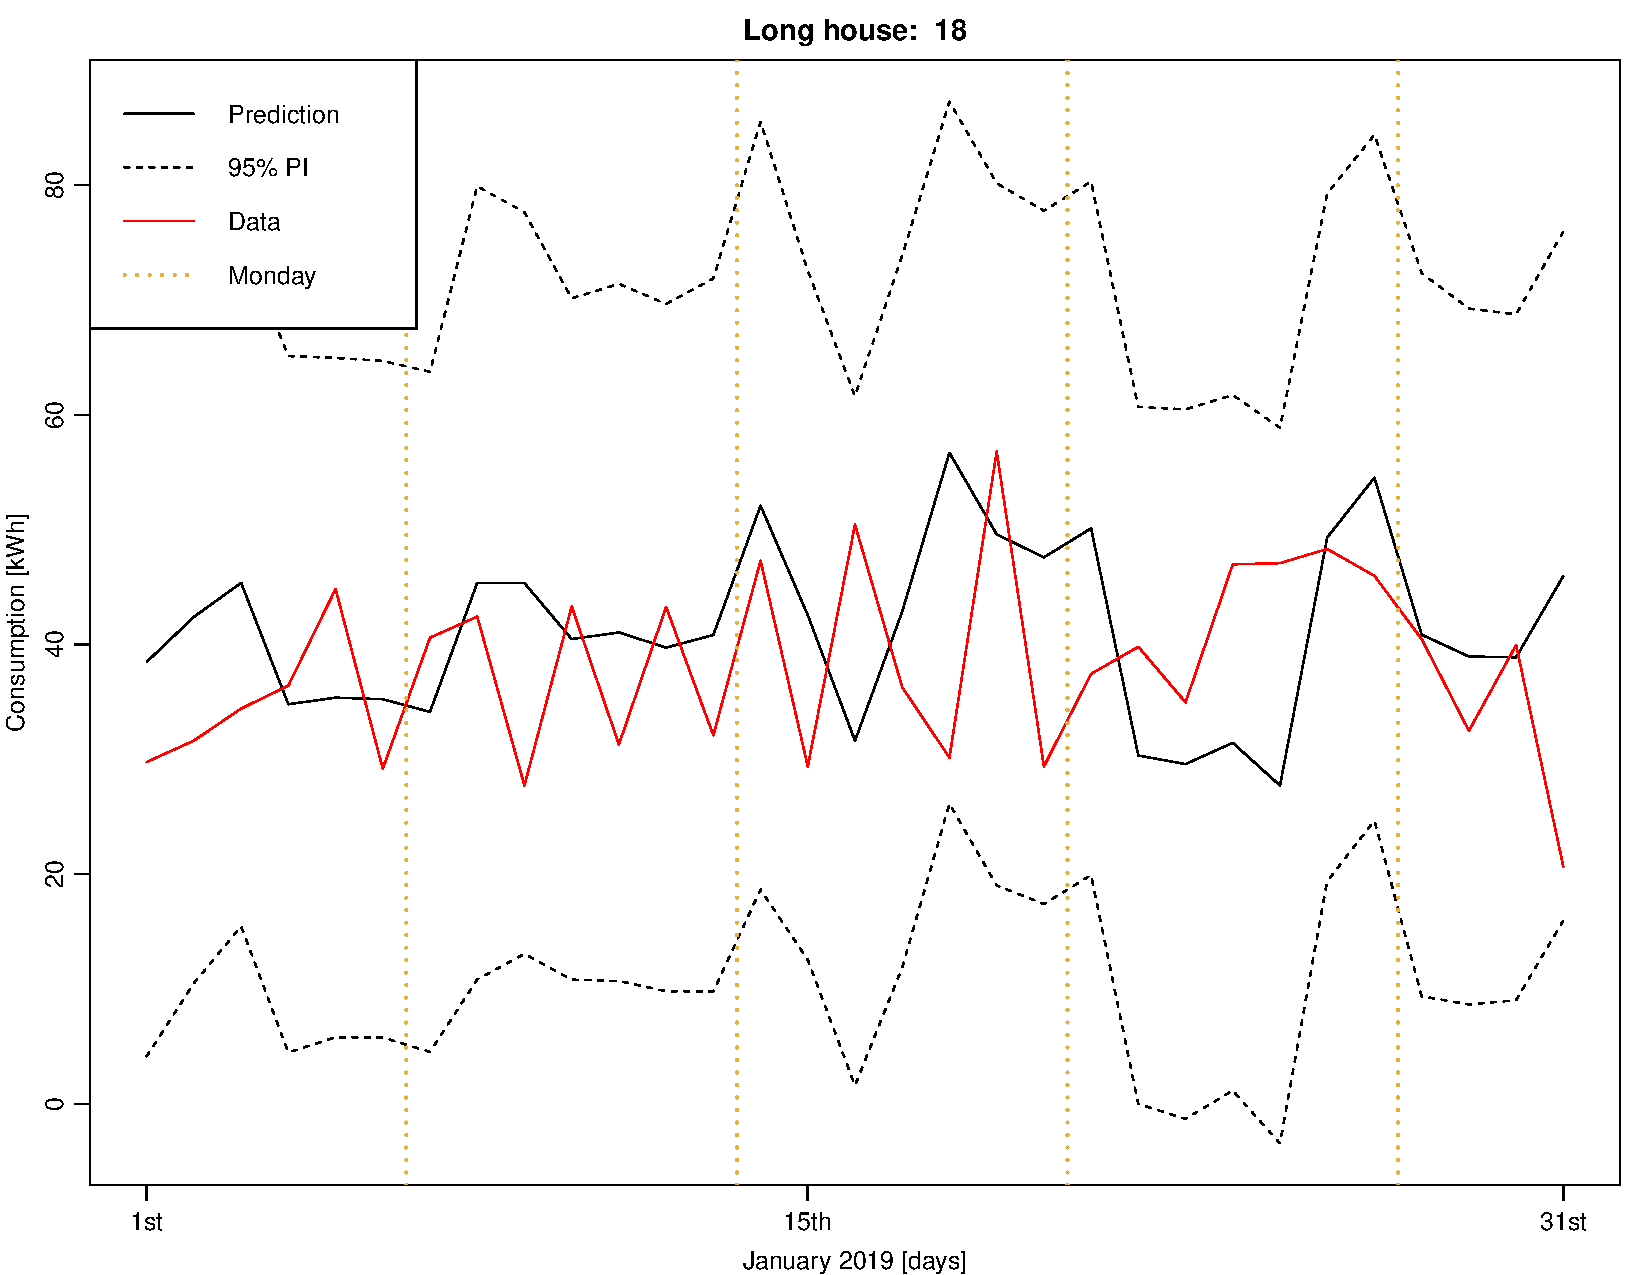
\includegraphics[width=.8\textwidth]{../../../figures/lmpred_18L.pdf}
    \caption{}
    \label{fig: lmpred_18L}
\end{figure}
\begin{figure}
    \centering
    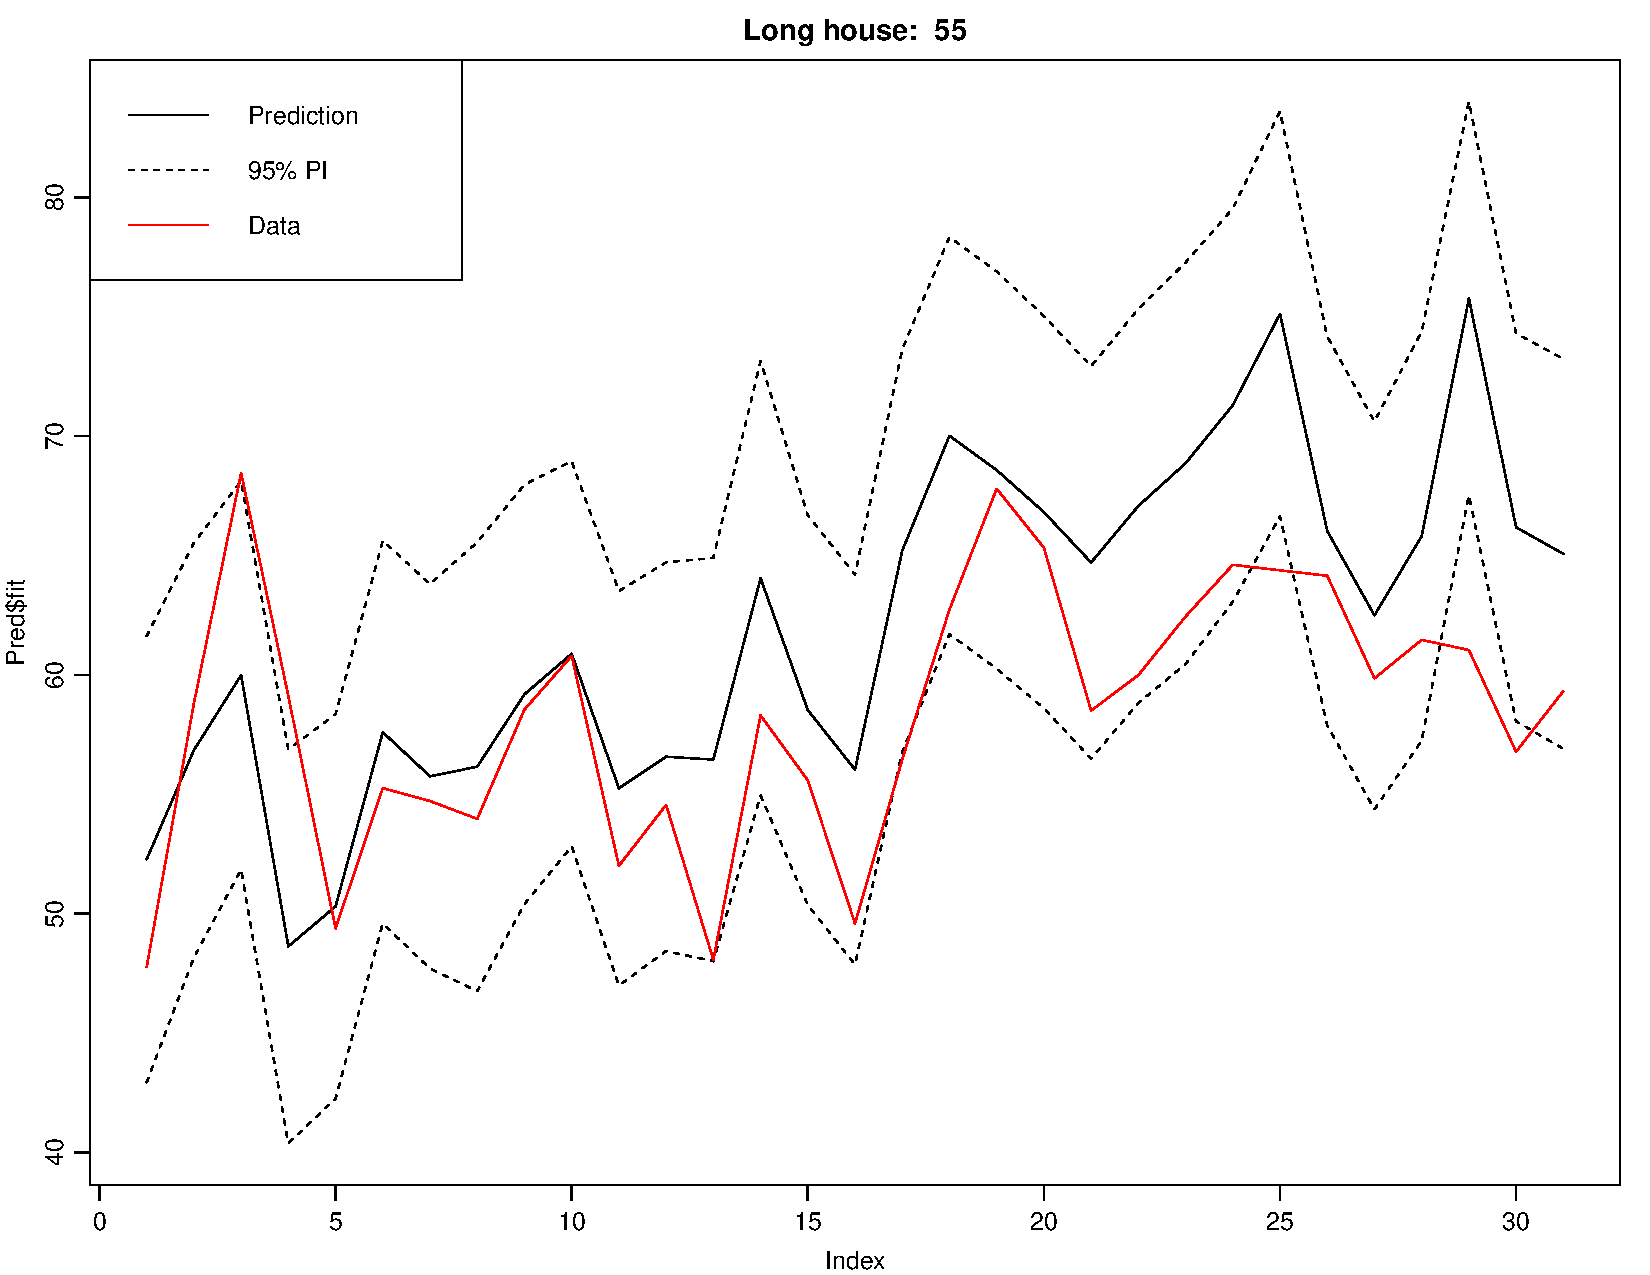
\includegraphics[width=.8\textwidth]{../../../figures/lmpred_55L.pdf}
    \caption{}
    \label{fig: lmpred_55L}
\end{figure}

\section{Comparison}
\textcolor{red}{Noget med at vi forventede den multiple model ville være bedre i tests end den simple.}
